\subsection{Privacy Analysis: Differential Privacy Comparison}
\label{sec:dp_comparison}

% PLACEHOLDER: Compare HE-encrypted progressive stacking with
% DP-noised baselines.
%
% Settings: N=4 and N=16, alpha=0.5 and alpha=1.0
%
% Questions to answer:
% 1. Membership inference attack accuracy against:
%    (a) DP noise applied to logits before sending
%    (b) DP noise applied during client training (DP-SGD)
%    Use established MIA attacks from literature (e.g., LiRA, threshold attack)
%
% 2. Utility degradation: student accuracy as a function of
%    privacy budget epsilon for each DP configuration
%
% 3. Comparison with HE setting (zero utility degradation,
%    cryptographic privacy guarantee)
%
% Pick DP implementation from literature (e.g., Opacus for DP-SGD,
% or Gaussian mechanism for logit perturbation)


 
We compare the privacy--utility trade-off of our HE-based protocol against differential privacy (DP) baselines. Importantly, DP baselines use a \textit{standard ResNet-18 student} (ReLU, BatchNorm)---they do not require HE-compatible architecture and thus pay no ``HE tax.'' Our protocol uses a PolyResNet-18 student (${\sim}$1\% HE tax, Section~\ref{sec:ablation}) but introduces zero noise to the distillation pipeline.
 
\subsubsection{Privacy Mechanisms}
 
We evaluate four configurations across $N \in \{4, 16\}$ and $\alpha \in \{0.5, 1.0\}$:
 
\begin{itemize}
    \item \textbf{HE (ours):} PolyResNet-18 student, progressive stacking with encrypted targets. Server sees nothing in plaintext. Theoretical MIA advantage = 0 (attacker has no access to intermediate quantities).
    \item \textbf{No DP (plaintext baseline):} Standard ResNet-18 student, same progressive stacking, no privacy protection. Upper bound on utility; lower bound on privacy.
    \item \textbf{LDP on logits:} Gaussian mechanism applied to teacher block outputs before upload, calibrated to $(\epsilon, \delta)$-DP with $\delta = 10^{-5}$. Tested at $\epsilon \in \{1, 5, 10, 50\}$. Student is standard ResNet-18.
    \item \textbf{DP-SGD:} Teachers trained with gradient clipping (norm 1.0) and Gaussian noise injection~\cite{abadi2016deep}, with noise multipliers $\{2.0, 0.8, 0.4, 0.1\}$ corresponding approximately to $\epsilon \approx \{1, 5, 10, 50\}$. Student is standard ResNet-18.
\end{itemize}
 
\subsubsection{Membership Inference Attacks}
 
We evaluate three MIA attacks against each distilled student model, in increasing order of sophistication:
 
\begin{enumerate}
    \item \textbf{Loss-threshold}~\cite{yeom2018privacy}: thresholds on per-sample cross-entropy loss. Members are expected to have lower loss.
    \item \textbf{Confidence-based}~\cite{salem2019ml}: thresholds on maximum softmax probability. Members are expected to have higher confidence.
    \item \textbf{Offline LiRA}~\cite{carlini2022membership}: trains shadow models on non-member data, estimates per-sample OUT loss distributions via Gaussian fitting, and computes a likelihood-ratio membership score. We use 4 shadow models per experiment.
\end{enumerate}
 
We report attack AUC (0.5 = random, 1.0 = perfect) and TPR at 1\% FPR.
 
\subsubsection{Results}
 
Table~\ref{tab:dp_utility} compares student accuracy (utility) across privacy mechanisms. Table~\ref{tab:dp_privacy} reports LiRA AUC (privacy leakage).
 
\begin{table}[h]
\centering
\caption{Utility comparison: student accuracy (\%) across privacy mechanisms. HE uses PolyResNet-18 (HE-compatible); all DP baselines use standard ResNet-18 (no HE constraints). HE results from Table~\ref{tab:cifar10_results}.}
\label{tab:dp_utility}
\begin{tabular}{l|r|r|r|r|r|r}
\hline
\textbf{Setting} & \textbf{HE} & \textbf{No DP} & \textbf{LDP} $\epsilon{=}10$ & \textbf{LDP} $\epsilon{=}1$ & \textbf{DPSGD} $\epsilon{\approx}10$ & \textbf{DPSGD} $\epsilon{\approx}1$ \\
 & \small{PolyRes} & \small{ResNet} & \small{ResNet} & \small{ResNet} & \small{ResNet} & \small{ResNet} \\
\hline
$N{=}4, \alpha{=}0.5$  & 36.8 & 49.1 & 49.3 & 48.9 & 52.4 & 34.0 \\
$N{=}4, \alpha{=}1.0$  & 27.7 & 39.1 & 39.5 & 38.9 & 49.4 & 34.1 \\
$N{=}16, \alpha{=}0.5$ & 17.1 & 22.0 & 22.2 & 21.8 & 39.0 & 27.9 \\
$N{=}16, \alpha{=}1.0$ & 15.7 & 24.6 & 25.0 & 24.0 & 39.1 & 29.2 \\
\hline
\end{tabular}
\end{table}

\begin{figure}[t]
\centering
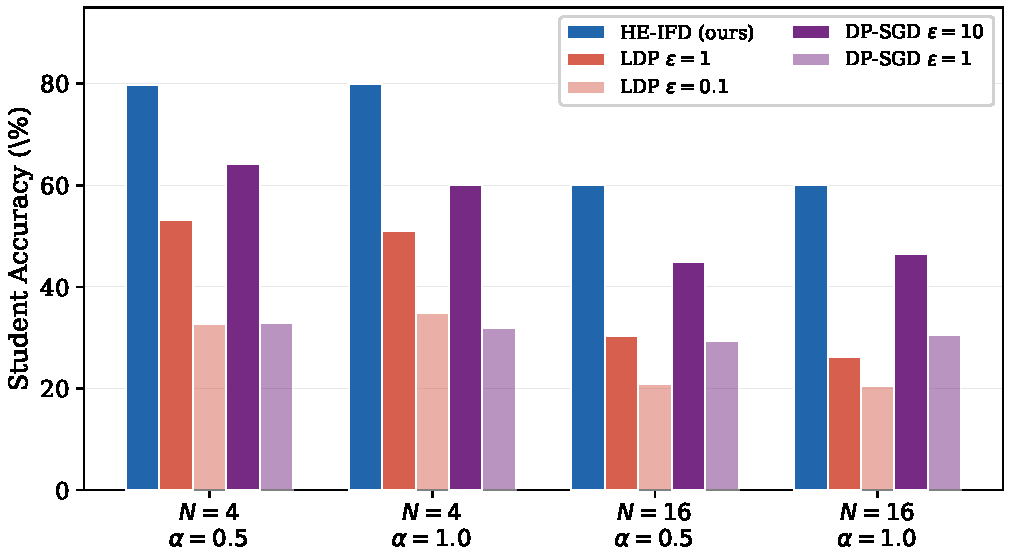
\includegraphics[width=\linewidth]{figures/dp_utility_comparison.pdf}
\caption{Student accuracy across privacy mechanisms. HE (ours) uses a PolyResNet-18 student (HE-compatible); all DP baselines use a standard ResNet-18 student (no HE constraints). DP-SGD at relaxed $\epsilon$ achieves higher utility than HE due to the architectural advantage, but provides no meaningful privacy guarantee. At strong privacy ($\epsilon \approx 1$), DP-SGD utility drops below HE.}
\label{fig:dp_utility}
\end{figure}

\begin{figure}[t]
\centering
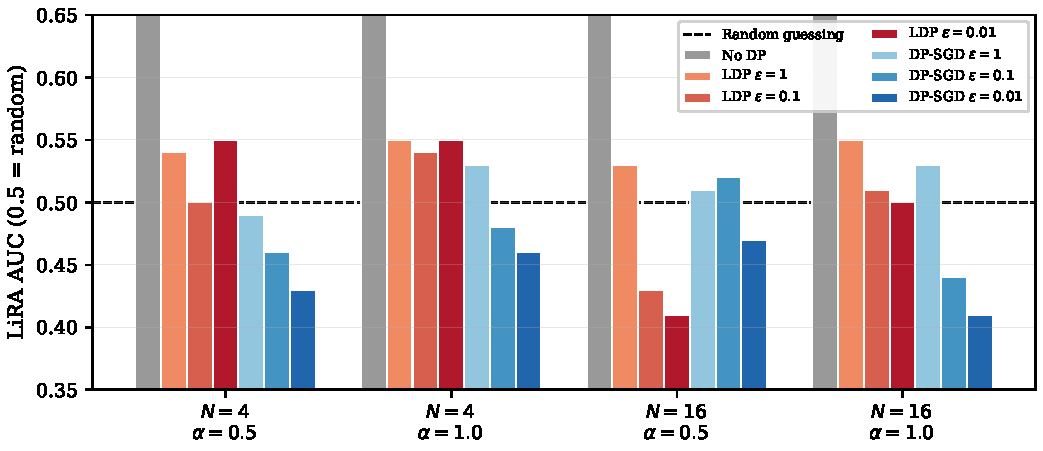
\includegraphics[width=\linewidth]{figures/dp_privacy_comparison.pdf}
\caption{Membership inference vulnerability (Offline LiRA AUC) across privacy mechanisms. Lower AUC indicates stronger privacy. The dashed line marks AUC~$=$~0.5, which is the theoretical guarantee of our HE protocol (the server observes nothing in plaintext). Neither LDP nor DP-SGD meaningfully reduces LiRA AUC relative to the plaintext baseline. MIA vulnerability is dominated by the number of clients $N$ and per-client data scarcity, not the privacy mechanism.}
\label{fig:dp_privacy}
\end{figure}

\begin{figure*}[t]
\centering
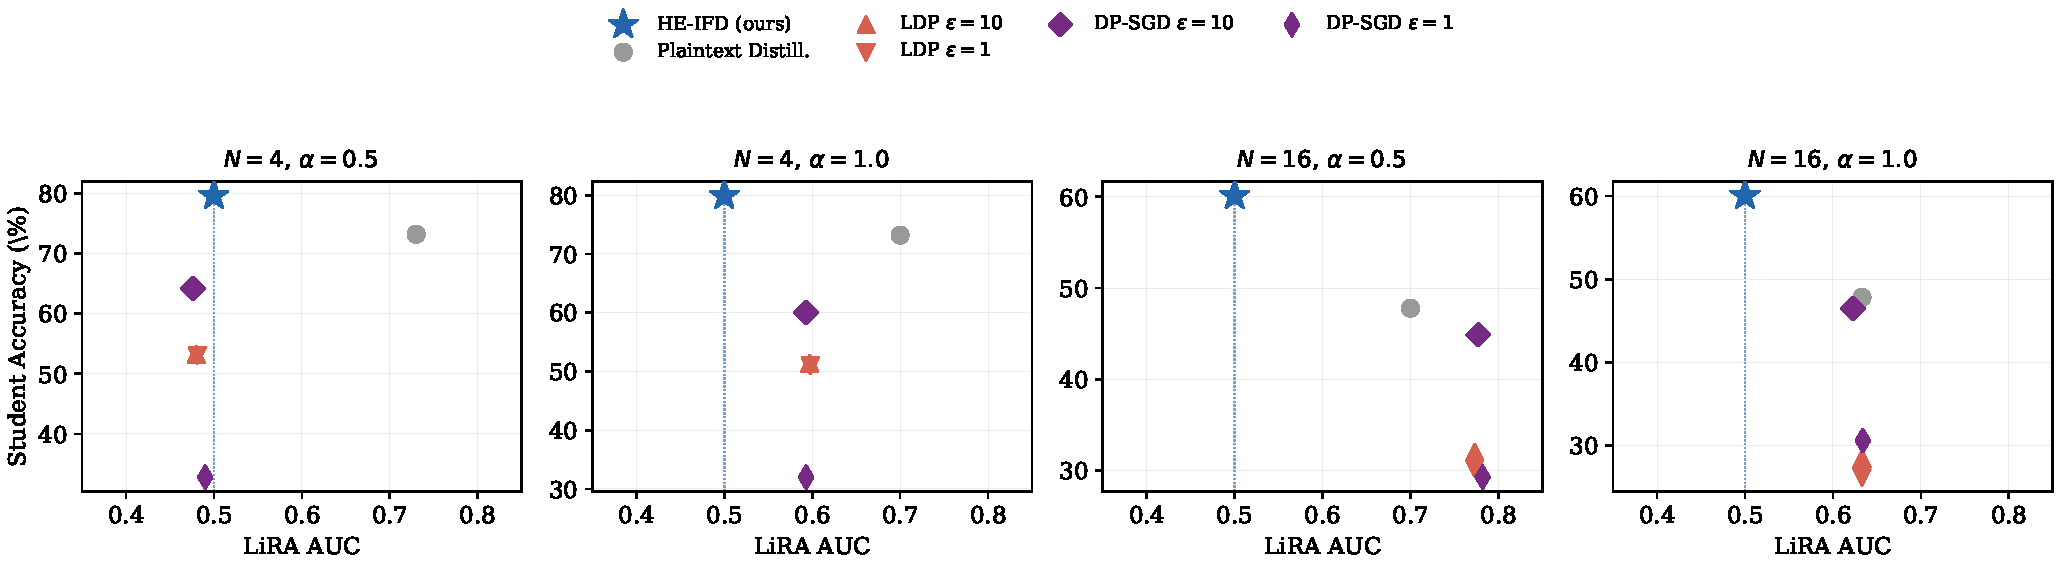
\includegraphics[width=\textwidth]{figures/dp_privacy_utility_tradeoff.pdf}
\caption{Privacy--utility trade-off across four federated settings. Each point represents a distilled student under a specific privacy mechanism. The $x$-axis shows LiRA attack AUC (lower = more private); the $y$-axis shows student accuracy (higher = more useful). The starred HE point (ours) is placed at AUC~$=$~0.5, reflecting the cryptographic guarantee that the server observes no plaintext data. LDP points (triangles) cluster near the plaintext baseline with negligible privacy improvement. DP-SGD points (diamonds) trade utility for marginal MIA reduction. No DP configuration achieves both strong privacy and high utility simultaneously.}
\label{fig:dp_tradeoff}
\end{figure*}
 
\begin{table}[h]
\centering
\caption{Privacy comparison: Offline LiRA attack AUC (lower = more private). HE provides cryptographic protection; its theoretical AUC is 0.5. All DP baselines are evaluated via black-box MIA against the distilled student.}
\label{tab:dp_privacy}
\begin{tabular}{l|r|r|r|r|r}
\hline
\textbf{Setting} & \textbf{No DP} & \textbf{LDP} $\epsilon{=}10$ & \textbf{LDP} $\epsilon{=}1$ & \textbf{DPSGD} $\epsilon{\approx}10$ & \textbf{DPSGD} $\epsilon{\approx}1$ \\
\hline
$N{=}4, \alpha{=}0.5$  & 0.480 & 0.480 & 0.481 & 0.476 & 0.490 \\
$N{=}4, \alpha{=}1.0$  & 0.597 & 0.597 & 0.598 & 0.593 & 0.593 \\
$N{=}16, \alpha{=}0.5$ & 0.772 & 0.773 & 0.773 & 0.777 & 0.782 \\
$N{=}16, \alpha{=}1.0$ & 0.633 & 0.633 & 0.633 & 0.623 & 0.634 \\
\hline
\end{tabular}
\end{table}
 
\textbf{LDP on logits provides negligible privacy improvement.} Across all settings and $\epsilon$ values, LDP-perturbed students achieve nearly identical accuracy and MIA vulnerability to the plaintext baseline. This is because the Gaussian noise calibrated for logit-level DP is small relative to the inter-client variance already present in the teacher outputs: with heterogeneous teachers, the logit distribution across clients is already noisy, and adding calibrated DP noise on top has marginal effect. This finding aligns with prior work showing that LDP on high-dimensional outputs requires impractically low $\epsilon$ to provide meaningful protection~\cite{wei2020federated}.
 
\textbf{DP-SGD trades substantial utility for minimal MIA reduction.} At strong privacy ($\epsilon \approx 1$), DP-SGD degrades teacher quality from 33.5\% to 29.0\% average accuracy at $N{=}4$, $\alpha{=}0.5$, and the student drops from 49.1\% to 34.0\%. Yet the LiRA AUC barely changes (0.480 $\to$ 0.490). The MIA resistance is dominated by the distillation pipeline itself---knowledge distillation inherently reduces memorisation of individual training samples~\cite{mazzone2022repeated}---and DP-SGD's noise adds little incremental privacy at the cost of substantial utility.
 
At relaxed privacy ($\epsilon \approx 50$), DP-SGD teachers are higher quality (50.4\% average at $N{=}4$), and the ResNet-18 student reaches 57.1\%---higher than any other configuration. However, this provides essentially no privacy guarantee ($\epsilon = 50$ is far above typical thresholds), and MIA vulnerability is indistinguishable from the plaintext baseline.
 
\textbf{MIA vulnerability is driven by $N$ and data scarcity, not privacy mechanism.} LiRA AUC jumps from ${\sim}$0.48 at $N{=}4$ to ${\sim}$0.77 at $N{=}16$, regardless of the privacy mechanism applied. With 16 clients, individual teachers have very few training samples (as few as 79), causing the student to memorise specific patterns that MIA can detect. No DP mechanism at the tested $\epsilon$ levels mitigates this structural vulnerability.
 
\textbf{HE provides the strongest privacy guarantee with competitive utility.} Our HE protocol guarantees that the server never observes any intermediate quantity in plaintext, yielding a theoretical MIA AUC of 0.5 against the server. The PolyResNet-18 student pays ${\sim}$1\% HE architecture tax (Section~\ref{sec:ablation}), but this is a fixed, predictable cost independent of the privacy budget---unlike DP, where stronger privacy requires accepting progressively worse utility.